\begin{figure}[t]
\newcommand{\figwidth}{1.7in}
\begin{center}
  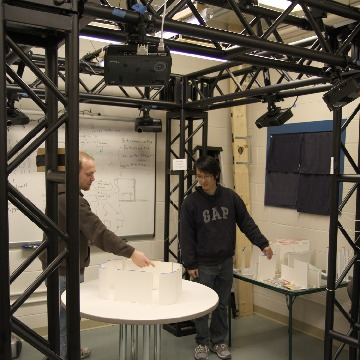
\includegraphics[width=\figwidth]{josh_jonathan_new_contraption}
  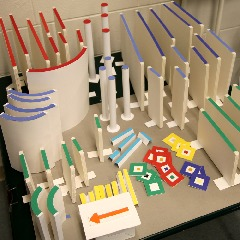
\includegraphics[width=\figwidth]{available_wall_pieces}\vspace{-0.19in}\\
\begin{minipage}{\figwidth}~{\color{white}{\bf a)}}\end{minipage}
\begin{minipage}{\figwidth}~{\color{white}{\bf b)}}\end{minipage}\vspace{0.05in}\\
  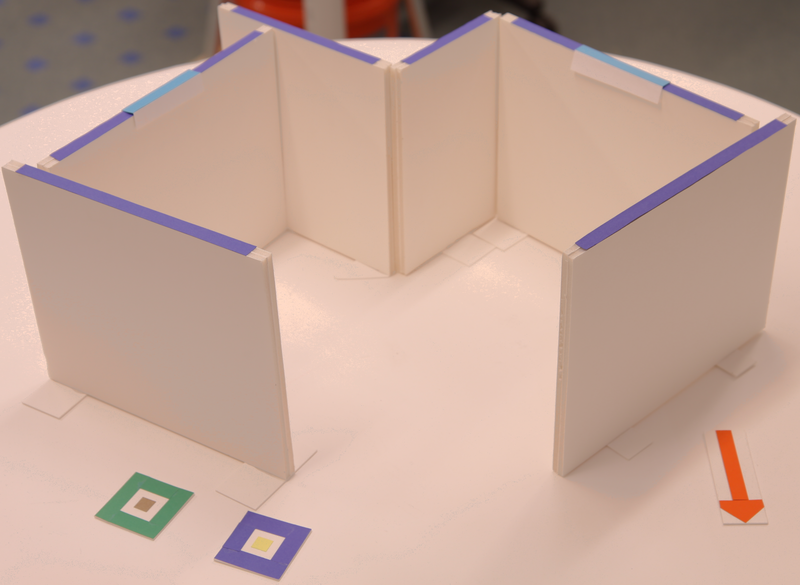
\includegraphics[width=\figwidth]{sample_model}
  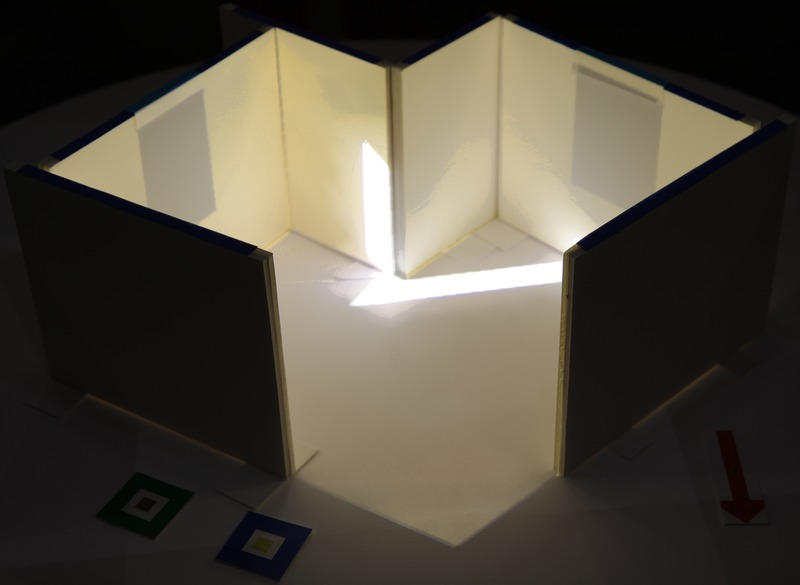
\includegraphics[width=\figwidth]{sample_rendering}\vspace{-0.19in}\\
\begin{minipage}{\figwidth}~{\color{black}{\bf c)}}\end{minipage}
\begin{minipage}{\figwidth}~{\color{white}{\bf d)}}\end{minipage}\vspace{-0.15in}\\
\end{center}
  \caption{Our new TUI for architectural daylighting design allows
    multiple users to a) gather around a physical sketching
    environment and select from b) a set of wall primitives and window
    and material markers to c) build a rough sketch of an
    architectural design.  A d) visualization of a daylighting
    simulation is projected onto these surfaces. 
	\label{figure:tabletop}
	}
  
\end{figure}
